\notechapter{N-20240824}{Riemann Surfaces: Complex Charts, Spheres, and Holomorphic Maps}

\section{Why Riemann surfaces are geometry}

A Riemann surface is a one-dimensional complex manifold. Since one complex dimension equals two real dimensions, it is a surface with complex coordinates.

The definition is local: every point has a neighborhood that looks like an open set in \(\mathbb C\), and the coordinate changes are holomorphic.

The surprise is that this small condition ties together topology, complex analysis, and algebraic geometry.

\section{Complex charts}

A complex chart is a homeomorphism
\[
  \varphi:U\to V\subset\mathbb C.
\]
Two charts \(\varphi\) and \(\psi\) are compatible if the transition function
\[
  \psi\circ\varphi^{-1}
\]
is holomorphic wherever it is defined.

A Riemann surface is a topological surface equipped with an atlas of such charts.

\section{The Riemann sphere}

The most important example is the Riemann sphere
\[
  \mathbb{CP}^1=\mathbb C\cup\{\infty\}.
\]
It has two standard charts. One uses the coordinate \(z\) on \(\mathbb C\). The other uses \(w=1/z\) near infinity. On the overlap, the transition map is \(w=1/z\), which is holomorphic away from \(0\).

\begin{figure}[H]
\centering
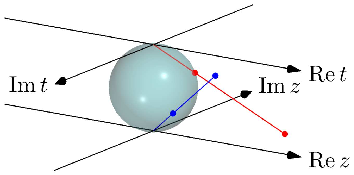
\includegraphics[width=.48\linewidth]{figures/N-20240824/riemsphere.pdf}
\caption{The Riemann sphere is the complex plane plus one point at infinity.}
\end{figure}

\section{Complex tori}

Let \(\Lambda\subset\mathbb C\) be a lattice, for example
\[
  \Lambda=\mathbb Z+\tau\mathbb Z,\qquad \operatorname{Im}\tau>0.
\]
The quotient \(\mathbb C/\Lambda\) is a complex torus. Topologically it is a torus, but it also has complex charts inherited from the plane.

This example shows that Riemann surfaces are not only subsets of \(\mathbb C\). They can be made by gluing and quotienting.

\begin{figure}[H]
\centering
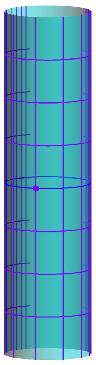
\includegraphics[width=.52\linewidth]{figures/N-20240824/CxCinf.pdf}
\caption{Complex geometry often comes from gluing local coordinate pictures.}
\end{figure}

\section{Holomorphic maps}

A map \(f:X\to Y\) between Riemann surfaces is holomorphic if it is holomorphic in local charts. That is, after choosing coordinates near \(p\in X\) and \(f(p)\in Y\), the map becomes an ordinary holomorphic function of one complex variable.

A meromorphic function on \(X\) is the same as a holomorphic map
\[
  X\to\mathbb{CP}^1.
\]
Poles are not failures of the map; they are points sent to \(\infty\).

\section{Local form and multiplicity}

A nonconstant holomorphic map between Riemann surfaces looks locally like
\[
  z\longmapsto z^m
\]
after choosing suitable coordinates. The integer \(m\ge1\) is the local multiplicity or ramification index.

If \(m=1\), the map is locally one-to-one. If \(m>1\), several sheets come together at the point.

\section{Zeros and poles}

If \(f\) is meromorphic near \(p\), then in a local coordinate \(z\) with \(z(p)=0\), it can be written as
\[
  f(z)=z^m u(z),
\]
where \(u(0)\ne0\). The integer \(m\) is the order of \(f\) at \(p\):
\[
  \operatorname{ord}_p(f)=m.
\]
If \(m>0\), \(f\) has a zero. If \(m<0\), \(f\) has a pole.

%% expanded-on-review

\section{The sphere as two glued planes}

The Riemann sphere can be understood by gluing two copies of \(\mathbb C\). Let one chart have coordinate \(z\), and the other have coordinate \(w\). On the overlap, identify them by
\[
  w=\frac1z.
\]
The point \(z=0\) in the first chart corresponds to \(w=\infty\), which is not in the second chart. The point \(w=0\) in the second chart is the point \(z=\infty\) in the first.

This gluing viewpoint is more flexible than the picture of a round sphere. It prepares the later idea that spaces can be built from coordinate patches and transition functions.

\section{Algebraic curves as Riemann surfaces}

A smooth complex plane curve often becomes a Riemann surface. For example, the affine curve
\[
  y^2=x^3-x
\]
can be completed by adding points at infinity, and the resulting smooth projective curve is a compact Riemann surface.

This is one of the central bridges in geometry:
\[
\begin{array}{c}
  \text{polynomial equations over }\mathbb C\\
  \Downarrow\\
  \text{complex curves}\\
  \Downarrow\\
  \text{Riemann surfaces}
\end{array}
\]
The same object may be studied algebraically, analytically, or topologically.

\section{A small example of ramification}

Consider the map
\[
  f:\mathbb{CP}^1\to\mathbb{CP}^1,\qquad f(z)=z^2.
\]
Near \(0\), it has local form \(z\mapsto z^2\), so the ramification index at \(0\) is \(2\). Near \(\infty\), using the coordinate \(w=1/z\), it also looks like \(w\mapsto w^2\). So \(\infty\) is also ramified.

This simple map already shows the basic phenomenon: a holomorphic map between surfaces may behave like a covering map almost everywhere, but with controlled branching at special points.



\section{The same surface in three languages}

A compact Riemann surface can often be viewed in three ways:
\[
\begin{array}{c|c}
\text{topological view} & \text{a surface with genus}\\
\text{analytic view} & \text{charts with holomorphic transition maps}\\
\text{algebraic view} & \text{a smooth projective complex curve}
\end{array}
\]
The power of the subject comes from moving between these views.  A map may be studied by local power series, a curve by polynomial equations, and the same object by its handles and covering spaces.


\section{What to remember}

Riemann surfaces are a gentle gateway into modern geometry. They are concrete enough to be drawn as surfaces, analytic enough to use holomorphic functions, and algebraic enough to connect with curves and divisors.

\[
  \text{a Riemann surface is a real surface whose local coordinates know complex analysis.}
\]
